% -*- latex -*-
% c4.tex
% LabSK 27.05.2022

% Wymagane pola (komentarz):
% Dawid Chmielewski				% Imię Nazwisko
% Maszyny i sieci wirtualne		% Temat ćwiczenia

\documentclass[a4paper,11pt]{article}

\usepackage[T1]{polski}
\usepackage[utf8]{inputenc}  			% Kodowanie pliku
\usepackage{pdfpages}

\hoffset=-3.0cm                         % Mniejszy lewy margines
\textwidth=18cm                         % szerzej
\evensidemargin=0pt

\voffset=-3cm                           % Mniejszy górny margines
\textheight=27cm                        % szerzej wzdłuż

\setlength{\parindent}{0pt}             % Paragraf od początku linii
\setlength{\parskip}{\medskipamount}    % Odstęp pomiędzy paragrafami
\raggedbottom                           % bez rozciągania strony

% Dodatkowe komendy
\newcommand\BS{\char`\\}                % \BS == back-slash
\newcommand\TY{\raise.17ex\hbox{$\scriptstyle\mathtt{\sim}$}}   % \TY == większa tylda w \tt

\thispagestyle{empty}			        % bez numeracji stron
\usepackage{enumerate}

\begin{document}
\title{ Sieci komputerowe - sprawozdanie z ćwiczenia 5. }
\author{ Dawid Chmielewski, numer indeksu: 311188 }
\date{24 maja 2022}

\maketitle{Temat ćwiczenia: Kreacja maszyn i sieci wirtualnych.}

\section{Ogólny cel ćwiczenia}

Tematem ćwiczenia była kreacja sieci wirtualnej oraz podłączenie do niej maszyny wirtualnej. Ćwiczenie zrealizowałem w maszynie wirtualnej (system Ubuntu), w której to wykreowałem kolejną maszynę wirtualną (Alpine)- była to więc wirtualizacja zagnieżdżona (ang. nested).

\section{Skrypt tworzący sieć wirtualną}
Kreacja sieci w moim przypadku sprowadzała się do stworzenia mostka o nazwie {\tt b0}, do którego podłączyłem interfejs dający połączenie z internetem- {\tt enp0s3}.

\begin{verbatim}
    #!/bin/sh
    
    sudo ip link add b0 type bridge
    sudo ip addr flush dev enp0s3
    sudo ip link set dev enp0s3 master b0
    sudo ip link set dev b0 up
    sudo dhclient b0
    sudo ip address add dev enp0s3 10.0.2.15/24
    
\end{verbatim}

\section{Skrypt tworzący maszynę wirtualną}

Maszyna tworzona przeze mnie chrakteryzuje się następującymi parametrami: 
\begin{itemize}

    \item nazwa- labsk5,

    \item 3 rdzenie procesora z pełnym ich wykorzystaniem,
    
    \item 512 MB pamięci RAM,
    
    \item system Alpine, którego obraz pobrałem wcześniej i zamontowałem jako dysk dvd.

\end{itemize}

Maszynę podpinam do mostka b0, który został utworzony w ramach poprzedniego skryptu.

{\tt
\begin{verbatim}
    #!/bin/sh
    
    vboxmanage unregistervm labsk5 --delete
    vboxmanage createvm --name labsk5 --register
    vboxmanage modifyvm labsk5 --memory 512 --vram 16
    vboxmanage modifyvm labsk5 --cpus 3
    vboxmanage modifyvm labsk5 --nictype1 virtio --nic1 bridged 
    --bridgeadapter1 b0 --nicbootprio1 1
    vboxmanage storagectl labsk5 --name IDE --add ide
    vboxmanage storageattach labsk5 --storagectl IDE --port 0 
    --device 0 --type dvddrive --medium "/home/dawid/alpine-standard-3.15.4-x86_64.iso"
    
\end{verbatim}
}

\section{Weryfikacja dostępu do internetu z poziomu gościa}

Do weryfikacji dostępu do internetu z maszyny użyłem domeny volt.zet.pw.edu.pl. Najpierw jednak musiałem dodać adres do interfejsu eth0, ustawić na nim bramkę domyślną oraz stworzyć plik resolv.conf i zapisać w nim adres serwera DNS:

{\begin{verbatim}

localhost:~# cat /etc/resolv.conf
nameserver 8.8.8.8

\end{verbatim}}

Poniżej prezentuję wyniki dla dwóch poleceń, których użyłem do diagnostyki połączenia sieciowego.

Za pomocą traceroute:

{\tt
\begin{verbatim}

localhost:~# traceroute volt.zet.pw.edu.pl -I
traceroute to volt.zet.pw.edu.pl (194.29.146.3), 30 hops max, 46 byte packets
 1  10.0.2.2 (10.0.2.2)  2.299 ms  1.943 ms  2.755 ms
 2  192.168.0.1 (192.168.0.1)  5.854 ms  5.491 ms  11.644 ms
 3  pl-waw10a-rt1.aorta.net (84.116.254.59)  22.181 ms  27.455 ms  31.964 ms
 4  *  *  *
 5  pl-gdn01a-rd1-ae-22-0.aorta.net (84.116.252.38)  25.844 ms  26.669 ms  28.440 ms
 6  212.191.238.224 (212.191.238.224)  27.118 ms  37.677 ms  26.495 ms
 7  212.191.238.192 (212.191.238.192)  33.617 ms  39.211 ms  35.478 ms
 8  212.191.238.193 (212.191.238.193)  33.033 ms  42.024 ms  45.170 ms
 9  148.81.253.70 (148.81.253.70)  35.878 ms  34.451 ms  36.667 ms
10  194.29.129.217 (194.29.129.217)  36.910 ms  38.514 ms  42.126 ms
11  194.29.129.234 (194.29.129.234)  77.782 ms  38.567 ms  36.886 ms
12  194.29.132.238 (194.29.132.238)  36.275 ms  *  42.115 ms
13  volt.iem.pw.edu.pl (194.29.146.3)  40.487 ms  41.272 ms  43.172 ms
14  volt.iem.pw.edu.pl (194.29.146.3)  32.021 ms  47.184 ms  42.870 ms

\end{verbatim}
}

Za pomocą ping:

{\tt
\begin{verbatim}
localhost:~# ping -c1 volt.zet.pw.edu.pl
PING volt.zet.pw.edu.pl (194.29.146.3): 56 data bytes
64 bytes from 194.29.146.3: seq=0 ttl=51 time=40.142 ms

--- volt.zet.pw.edu.pl ping statistics ---
1 packets transmitted, 1 packets received, 0% packet loss
round-trip min/avg/max = 40.142/40.142/40.142 ms
\end{verbatim}
}

\section{Test połączenia SSH}

Do połączenia się przez SSH musiałem na maszynie Alpine zainstalować pakiet OpenSSH: 

apk add openssh 

Następnie, edytując plik{\tt {\begin{verbatim} /etc/ssh/sshd_config \end{verbatim} } } odblokowałem dostęp do logowania się do root'a za pomocą hasła, na końcu zaś ustawiłem je za pomocą passwd.

Test połączenia SSH z maszyny Ubuntu na Alpine:

{\tt
\begin{verbatim}
dawid@dawid-VirtualBox:~/Desktop$ ssh root@10.0.2.17
root@10.0.2.17's password: 
Welcome to Alpine!

The Alpine Wiki contains a large amount of how-to guides and general
information about administrating Alpine systems.
See <http://wiki.alpinelinux.org/>.

You can setup the system with the command: setup-alpine

You may change this message by editing /etc/motd.

localhost:~#
\end{verbatim}
}

Z maszyny Alpine na Ubuntu:

{\tt
\begin{verbatim}
localhost:~# ssh dawid@10.0.2.15
dawid@10.0.2.15's password: 
Welcome to Ubuntu 22.04 LTS (GNU/Linux 5.15.0-33-generic x86_64)

 * Documentation:  https://help.ubuntu.com
 * Management:     https://landscape.canonical.com
 * Support:        https://ubuntu.com/advantage

109 updates can be applied immediately.
12 of these updates are standard security updates.
To see these additional updates run: apt list --upgradable

Last login: Fri May 27 21:29:12 2022 from 10.0.2.17
dawid@dawid-VirtualBox:~$ 
\end{verbatim}
}

\section{Minimalny schemat sieci}

Na następnej stronie prezentuję cały schemat. Mamy tutaj do czynienia z wirtualizacją
zagnieżdżoną, czyli maszyna wirtualna wewnątrz drugiej maszyny wirtualnej. Jest to dosyć ciekawa konfiguracja. Z moich spostrzeżeń czas konfiguracji maszyny zagnieżdżonej jest długi- nawet dla prostych systemów, jakim jest Alpine Linux.

\pagebreak
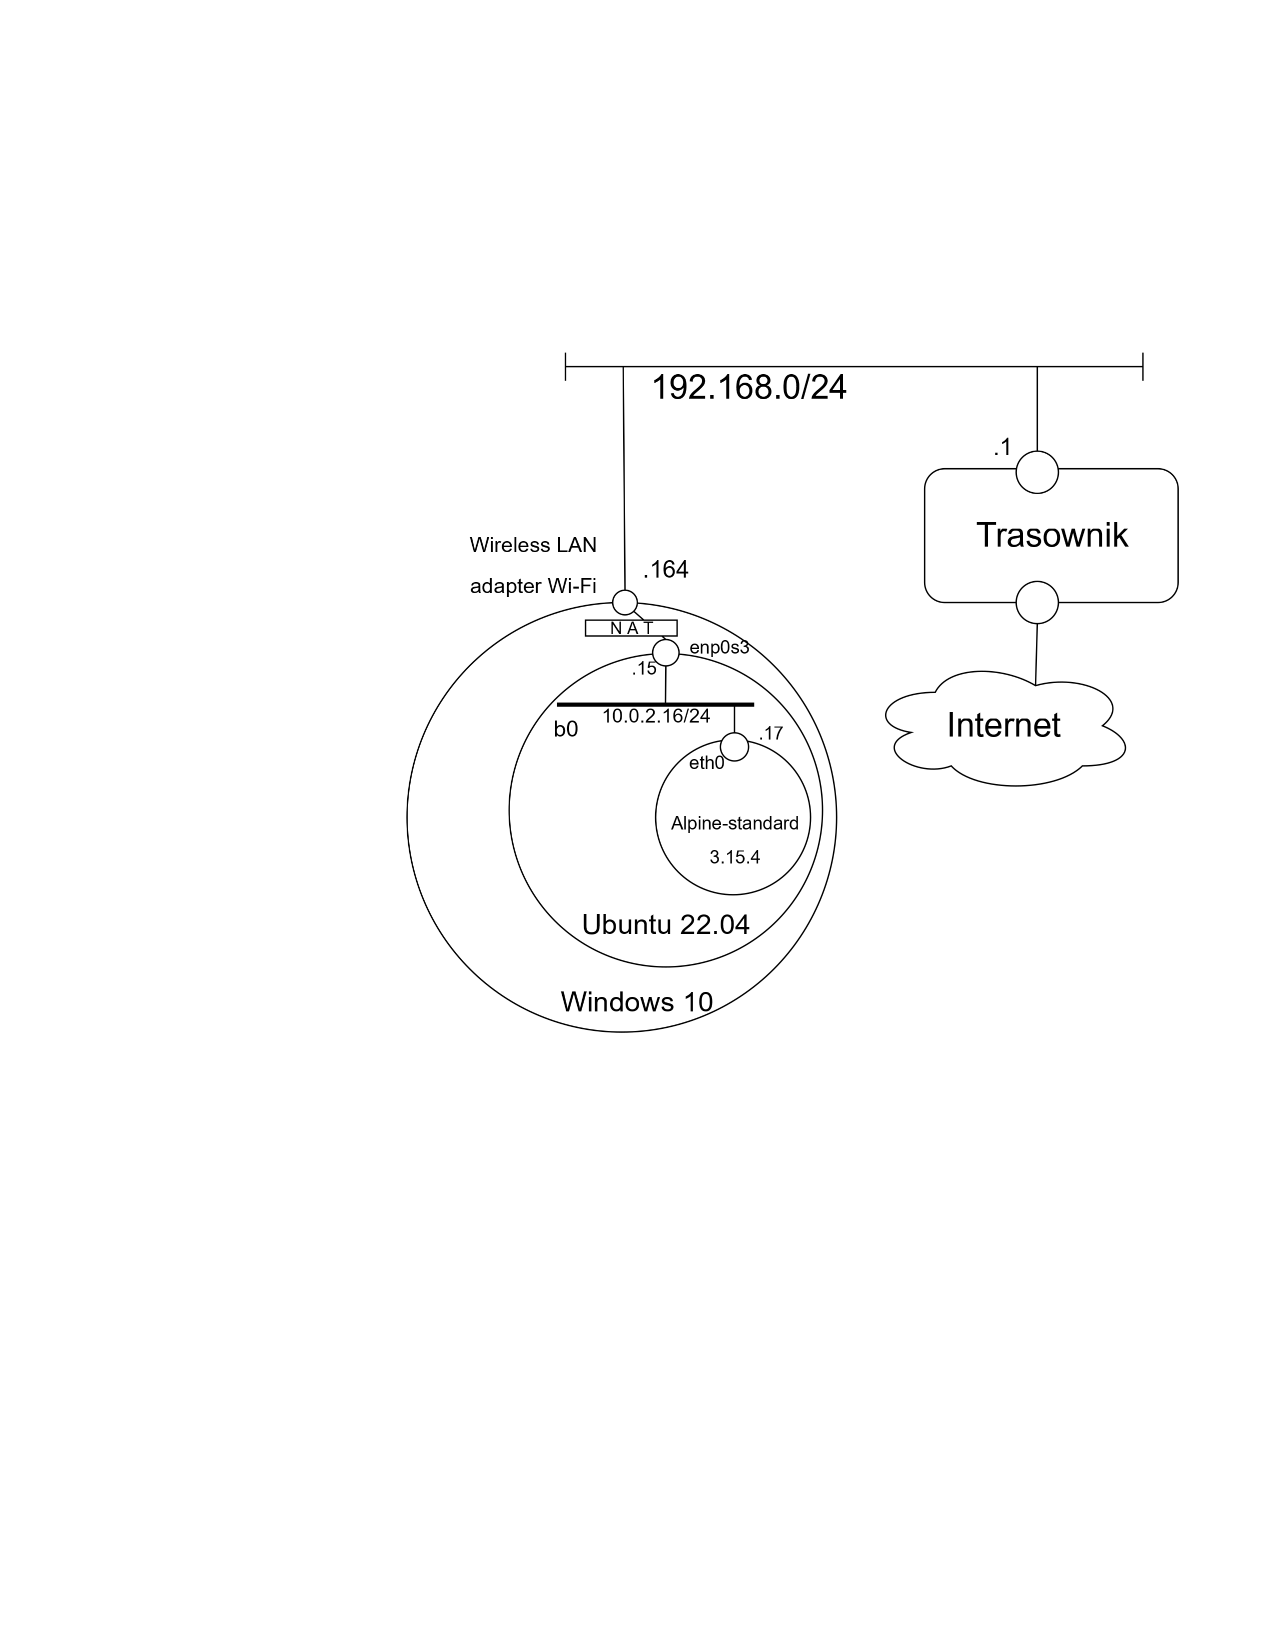
\includepdf[pages=-]{labsk5schemat.pdf}


\end{document}